% INTRODUCTION
%Editor: Xiaodong Jiang

\section{Introduction}
\label{sec:introduction}
The last two decades has seen remarkable progress in the knowledge 
of the polarized parton distribution functions (pPDF)
  $\Delta q_f(x)$.
The most precise and clearly interpreted data are from inclusive deep-inelastic
 lepton scattering (DIS)
experiments at CERN and SLAC. 
However, the information available from inclusive DIS process has inherent 
limitations.  As the cross 
sections are only sensitive to $e_q^2$, the quark charge square,
an inclusive experiment probes quarks and anti-quarks on an equal footing, and
 it is only possible to determine combinations of $\Delta q + \Delta \bar{q}$, 
but never the valence $\Delta q_v=\Delta q - \Delta \bar{q}$ nor the sea $\Delta \bar{q}$ separately.    
 Therefore it is not sensitive to the symmetry breaking in the sea sector. 
Through inclusive DIS measurements, only one particular flavor non-singlet can be directly 
inferred  i.e.  $\Delta q_{3}(x,Q^2)=\Delta u+\Delta \bar{u}-\Delta d-\Delta \bar{d}$. 
The additional assumption of SU(3)$_f$ flavor symmetry allows the hyperon beta decay data
to constrain the first moments of $\Delta q$.
The well-cited result of this approach is
that quark helicities seem to make a small net contribution to the nucleon spin, and the
strange sea appears to be negatively polarized.

Is sea quark polarized ?  This question has been tantalizing us for the last  two decades.  very recently, from RHIC STAR experiment's W-boson spin asymmetry measurements~\cite{Adamczyk:2014xyw}, as shown in Fig~\ref{fig:STAR_W}, the data strongly favor a positively polarized sea up-quark.  
% add more comments, and a figure here.
% STAR W paper and ubar positive polarization.
%%% Fig %%%

\begin{figure} [htbp]
  \centering
    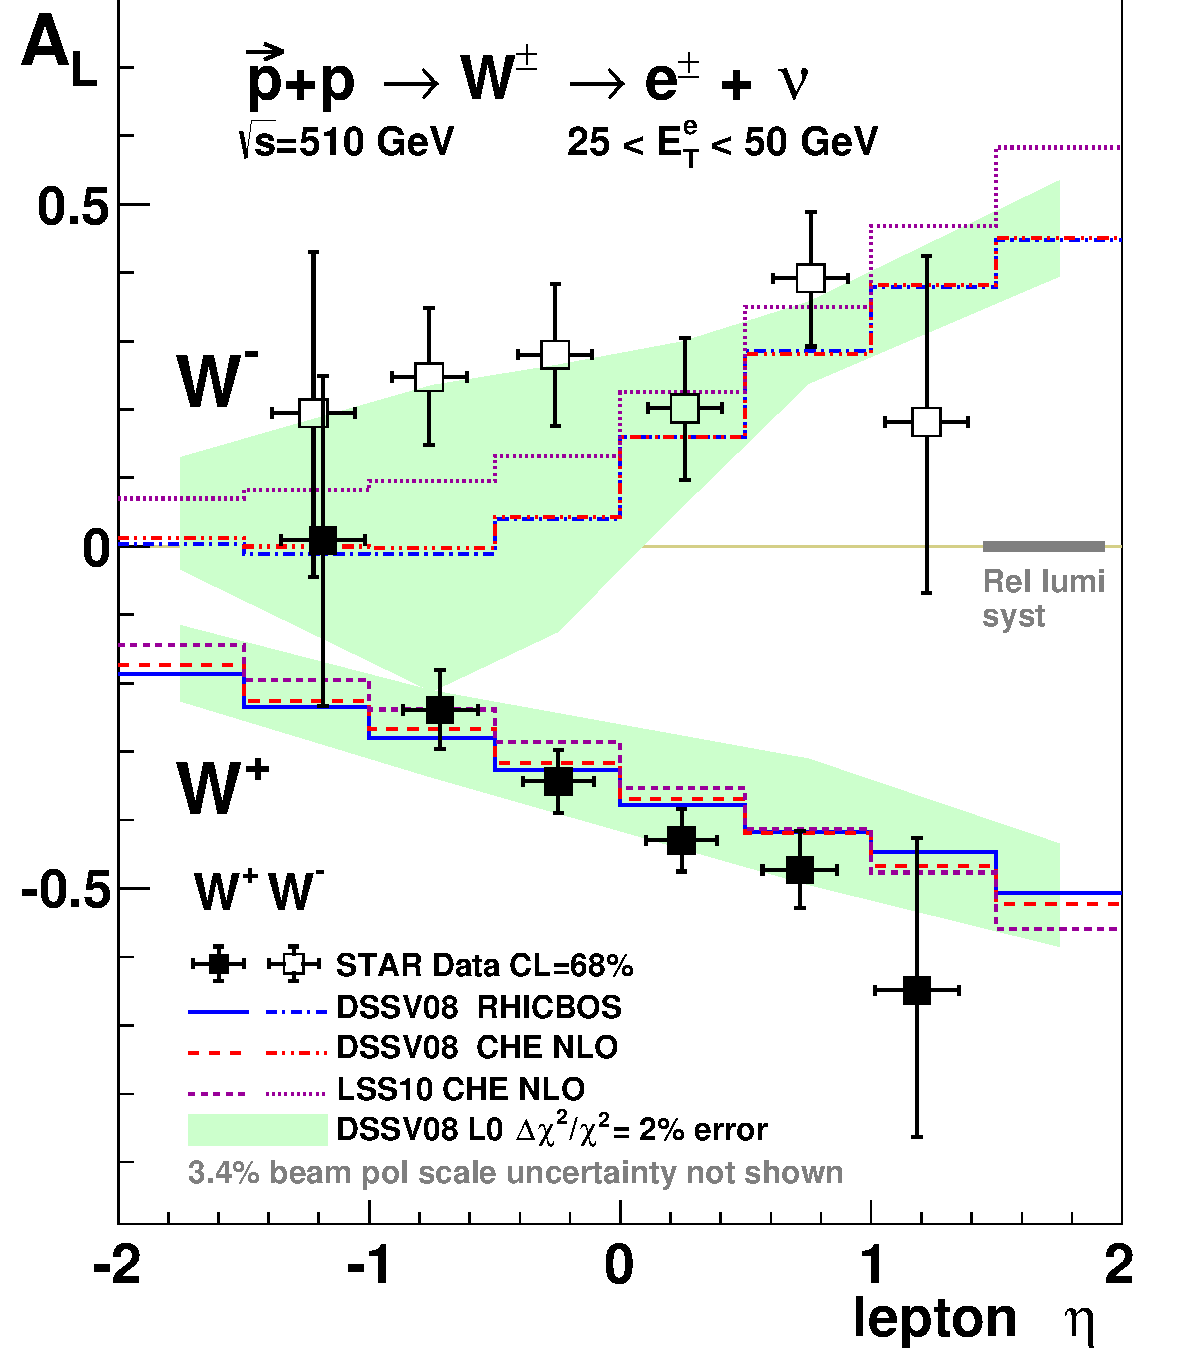
\includegraphics[width=0.50\linewidth]{figs_xj/STAR-WAL_2012.pdf}
    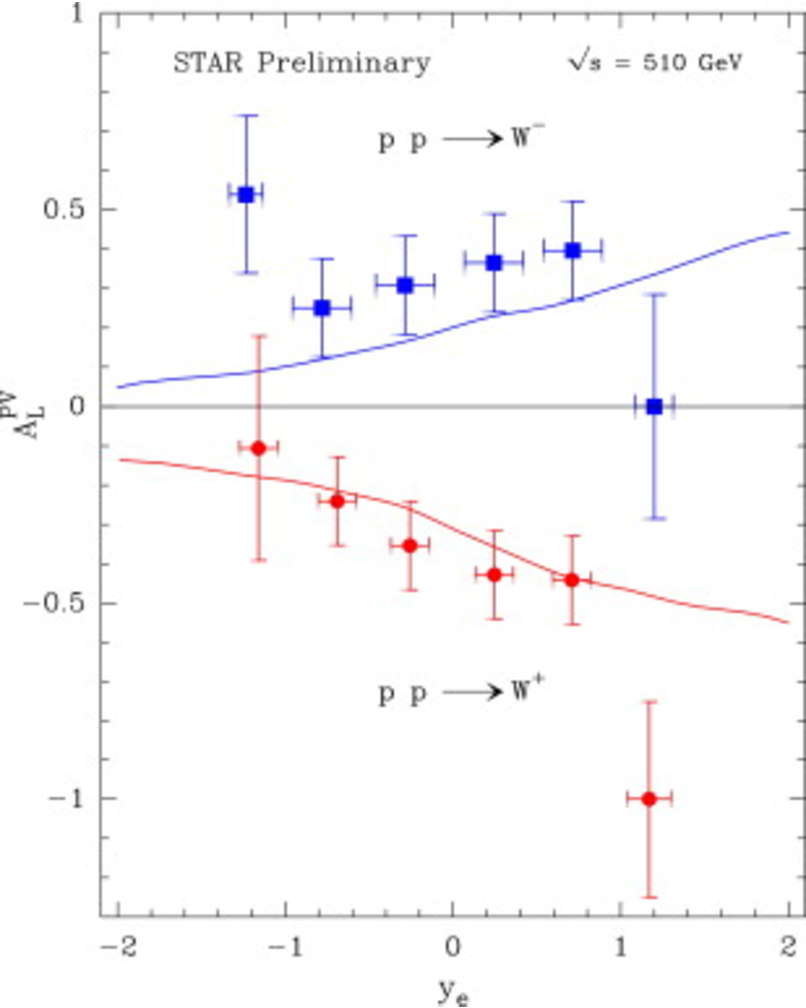
\includegraphics[width=0.47\linewidth]{figs_xj/BBS2008_STAR_Wpreliminary.pdf} \\
  \caption{\label{fig:STAR_W} (left)Recent results from STAR,  longitudinal single-spin asymmetry, $A_L$, for $W^\pm$ production as a function of lepton pseudorapidity, $\eta_e$, in comparison to theory predictions. (right need replaced) BBS2008 prediction compared with STAR preliminary data. }
\end{figure}

%BBS2008 ratios
\begin{figure} [htbp]
  \centering
    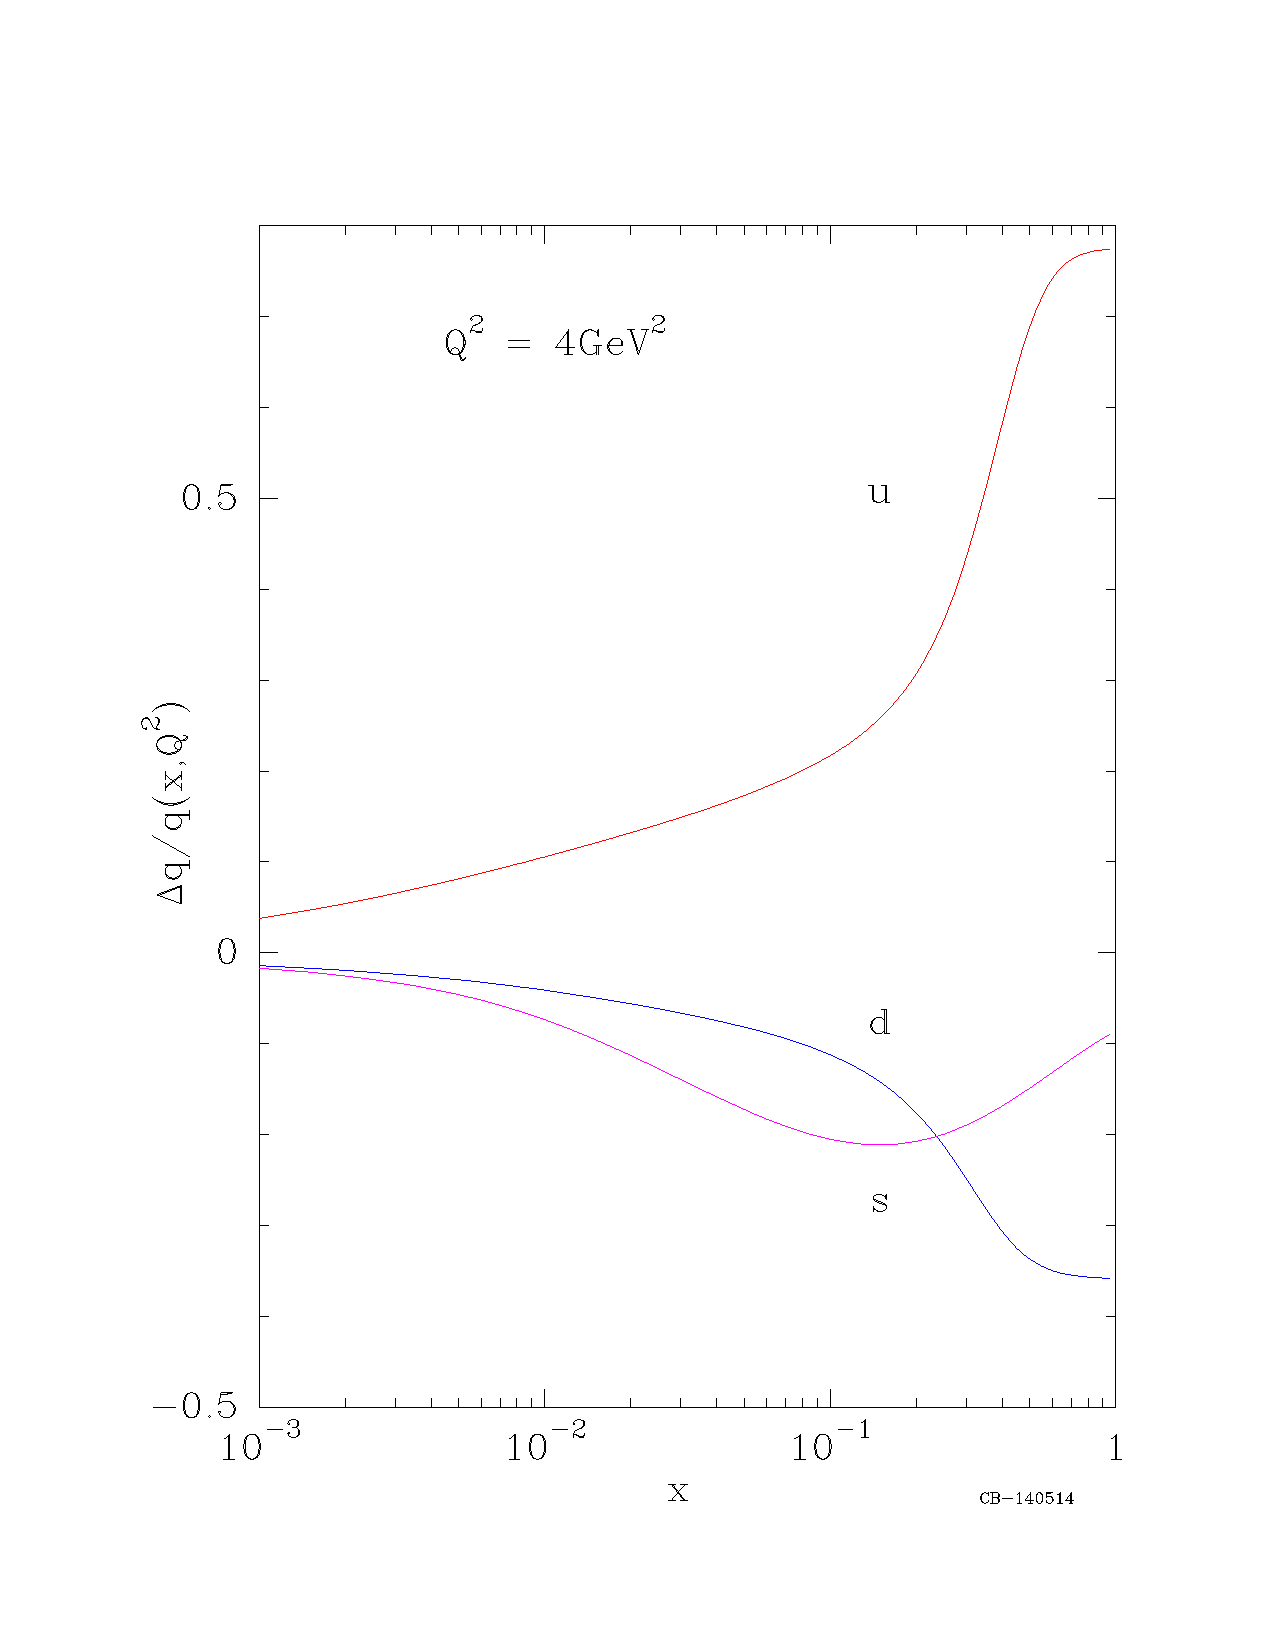
\includegraphics[width=0.49\linewidth]{figs_xj/BBS_deltaqoq.pdf}
    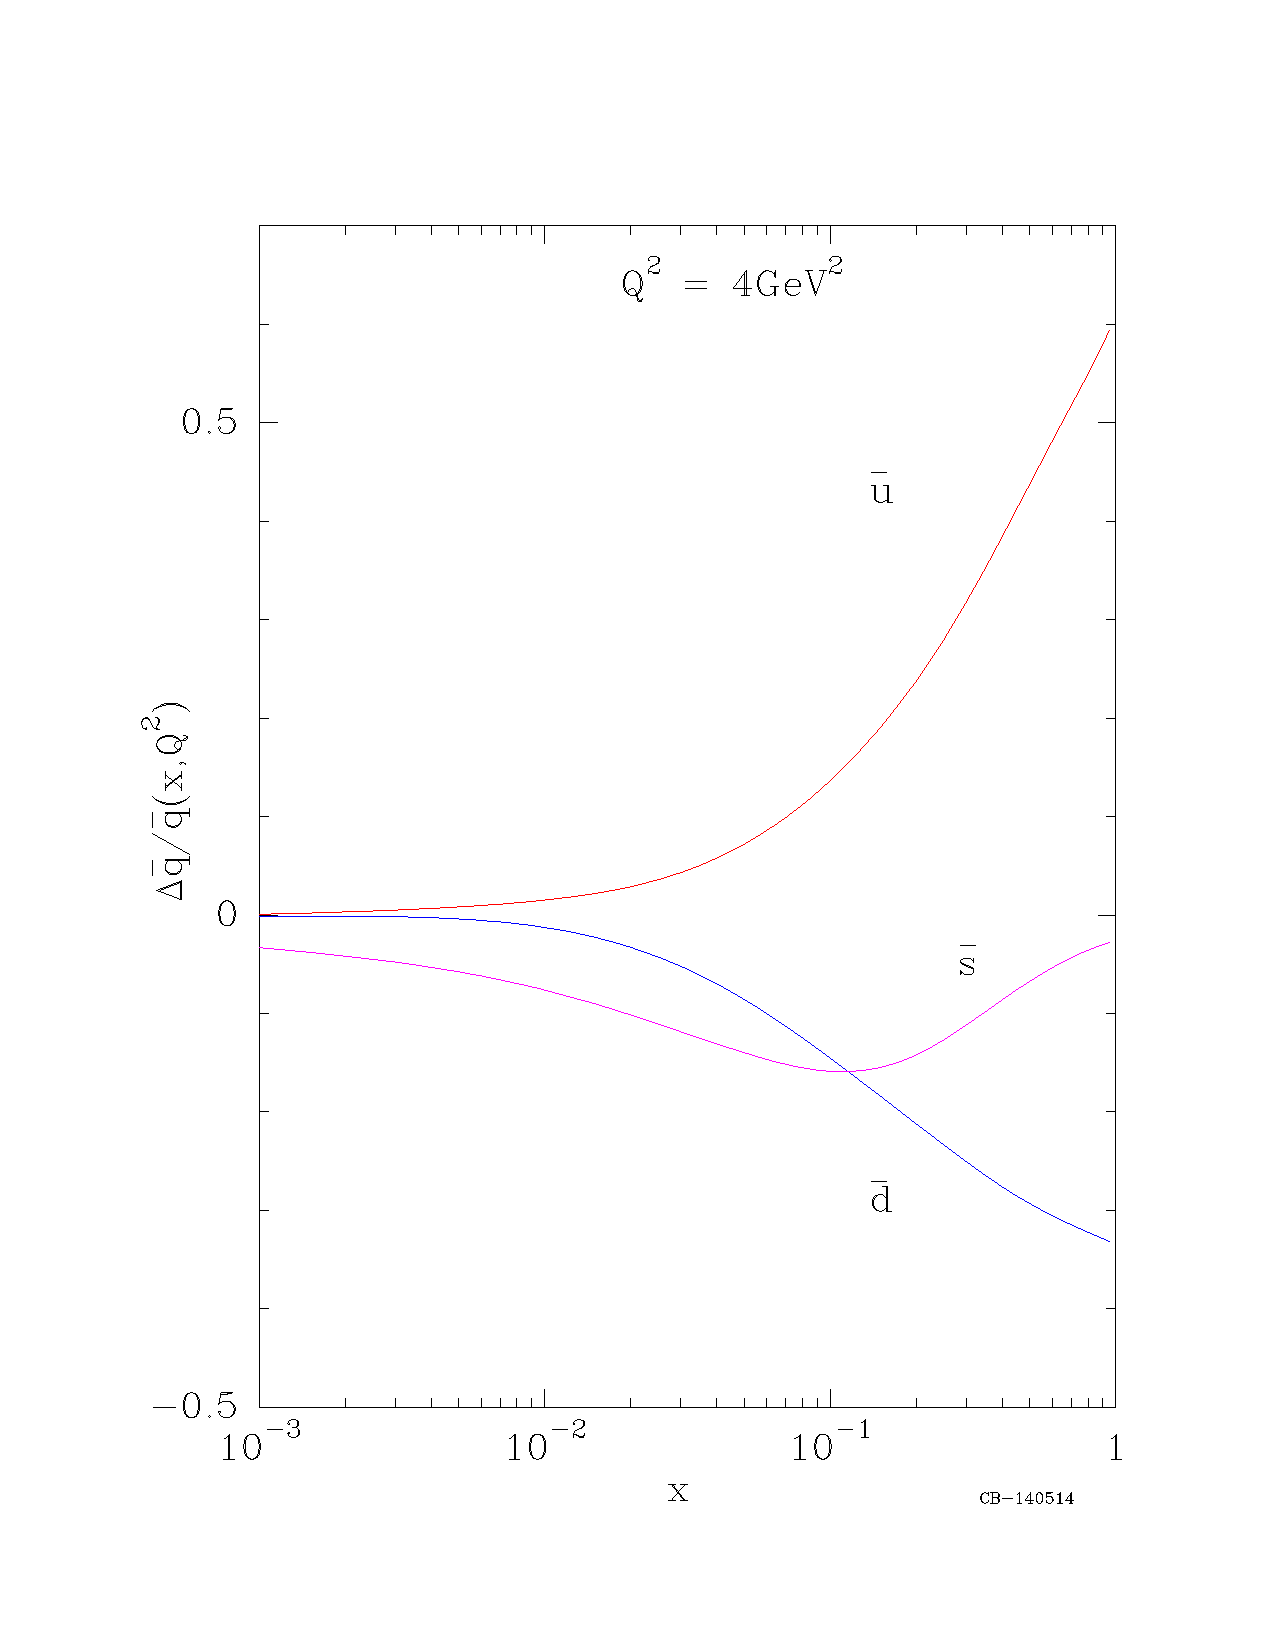
\includegraphics[width=0.49\linewidth]{figs_xj/BBS_deltaqbaroqbar.pdf} \\
  \caption{\label{fig:BBS_deltaqoq} BBS2008 prediction of raio for different quark flavor $\Delta q/q$  (left) and $\Delta \bar{q}/\bar{q}$ at the kinematics of this experiment $Q^2=4.0$ GeV$^2$.  }
\end{figure}

The sensitivity to each individual quark flavor can also be realized
in semi-inclusive deep inelastic scattering (SIDIS)
in which one of the leading hadrons in quark fragmentation is also detected.
Since the leading hadrons from the current fragmentation 
carry information about
the struck quark's flavor, detection of the leading hadron 
effectively ``tags'' the quark flavor.
Therefore, SIDIS offers an unique opportunity 
for determining the spin, flavor, and sea structure of the nucleon \cite{Frankfurt}, 
thereby significantly enriching 
our understanding of QCD and the nucleon structure. 
High precision polarized SIDIS data on the proton and the neutron 
(in a deuteron or a $^3$He nuclei) allows
a flavor decomposition of nucleon spin structure, which could lead to
the discovery of a possible flavor-asymmetry in the polarized sea.
A decade ago, in 2005, the HERMES collaboration
published the results of a leading order spin flavor decomposition from polarized 
proton and deuteron data, and for the first time
extracted the sea quark 
polarizations~\cite{hermes2002,hermesthesis}. Unlike 
the predictions of several theoretical models,
HERMES data indicated that within the available statistics
$\Delta \bar{u}- \Delta \bar{d}$ is consistent
with an unbroken SU(2)$_f$ symmetry.  These results have been confirmed in 2011 by the COMPASS Collaboration. 
%xj.  add citation COMPASS and comments here.  

The HERMES data demonstrated that, within the experimental precision, 
the semi-inclusive double-spin asymmetries $A_{1N}^h$ 
at $\langle Q^2 \rangle=2.5$ GeV$^2$ 
agree reasonably well with the 
SMC data~\cite{smc1998} at $\langle Q^2 \rangle=10$ GeV$^2$, COMPASS 
asymmetry data on deuteron~\cite{compass2007}, an proton targets  %COMPASS citation 
averaged at $\langle Q^2 \rangle=10$ GeV$^2$, was also shown to
agree well with HERMES data.

This non-trivial agreement indicates that semi-inclusive asymmetries have rather weak $Q^2$ dependencies and 
the expected violation of naive \lo $x$-$z$ separation is not large.  
The apparent ``precocious scaling'' suggests that at a modest $Q^2$, such as at HERMES $\langle Q^2 \rangle=2.5$ GeV$^2$ and 
at $\langle Q^2 \rangle=4.0$ GeV$^2$ for this experiment, information on the  quark distributions should be reasonably  
well-preserved in semi-inclusive reactions.   Ji, Ma and Yuan have  
explicitly proved~\cite{jimayuan04} that QCD factorization is valid for SIDIS with 
hadrons emitted in the current fragmentation region with low  
transverse momentum $p_{\perp h } \ll Q$.  QCD factorization of spin-dependent
cross sections in SIDIS and Drell-Yan has also been proved
 for the low $p_{\perp h }$ case~\cite{jimayuan04_2}.
JLab E00-108 data~\cite{rolf}, on unpolarized SIDIS cross section ratios
of proton and deuteron with 5.5 GeV beam and $\langle Q^2 \rangle=2.3$ GeV$^2$,  
also indicated that the leading order naive $x$-$z$ separation is
rather close to the reality. 

% NLO Global fits.

 It was  pointed out by Frankfurt et al.~\cite{Frankfurt} and by Christova and Leader~\cite{leader2} that 
if the yield-difference  helicity-asymmetries $A_{1N}^{\pi^+ - \pi^-}$ are measured with  high precision,
quark polarization $\Delta u_v$, $\Delta d_v$ and $\Delta \bar{u} - \Delta \bar{d}$ can be extracted
at \lo independent of the knowledge of fragmentation functions.  Even 
at the \nloo, information on the 
valence quark polarizations is well-preserved in the combined 
asymmetries $A_{1N}^{\pi^+ - \pi^-}$, due to the fact that contributions from 
gluons as well as sea-quarks cancel exactly to all orders of QCD~\cite{leader2} in this charge and flavor 
non-singlet combination.
In practice, the combined asymmetry $A_{1N}^{\pi^+ - \pi^-}$ poses more
experimental challenges, since precise knowledge on hadron phase spaces and detection 
efficiencies are required. This experiment is specifically designed to measure $A_{1N}^{\pi^+ - \pi^-}$.
Different from other SIDIS measurements like HERMES and COMPASS,
% and the planned CLAS12, 
this experiment will use two independent magnetic spectrometers. By flipping the magnetic 
polarity of the hadron spectrometer, identical phase spaces between $\pi^+$ and $\pi^-$ 
reaction can be achieved such that the combined asymmetry $A_{1He}^{\pi^+ - \pi^-}$ can be 
determined with high precision.
% in addition to the individual asymmetries $A_{1He}^h$. 
At $Q^2$ of $2.0\sim 6.7$ GeV$^2$, and $x=0.110 \sim 0.600$ ??? xxx.xx , this experiment will 
provide independent precision data on $\Delta d_v -{1 \over 4} \Delta u_v$.
When combined with the expected world data on polarized proton, 
%especially from the planned future CLAS12 experiment, 
to obtain $\Delta u_v - \Delta d_v$,
this experiment will provide the
opportunity to address the polarized sea asymmetry $\Delta \bar{u}- \Delta \bar{d}$. 

At the \nloo, following the well established formalism~\cite{PhysRevLett.101.072001},
tools of NLO QCD global fits, which include data sets from both inclusive and semi-inclusive reactions,
have become available.   As a standard procedure,  such global NLO QCD fit
has also included RHIC $pp$ data~\cite{deFlorian:2014yva}, in forward $\pi^0$ and jet longitudinal double-spin asymmetries $A_{LL}^{\pi^0}$, and $A_{LL}^{jet}$. 
Although there's a reasonable  set of SIDIS  data on proton and deuteron targets, from HERMES and COMPASS experiment, and soon from JLab-6GeV CLAS eg1-dvcs run group,  the world data on SIDIS asymmetries  currently only includes
one $^3$He data set, with rather large error bars, obtained by HERMES in 1996.
The high statistics $^3$He data from this experiment, adding much precise
 neutron SIDIS asymmetries to the world data sample,  
will serve as stringent constraints on pPDFs through NLO global fits~\cite{epjcxj2006}. 
Data from this experiment  will  indirectly constrain  $\Delta g$   through NLO global fit. 
The main source of this sensitivity to $\Delta g$ comes from 
the $Q^2$-evolutions of the inclusive $g_1$ structure function, but now with 
 sea and valence contributions much better
 separated by semi-inclusive data in the global fit~\cite{sassotnlo,epjcxj2006}.
Therefore,  data from this experiment will  independently verify 
the recent claim of a small positive gluon polarization based on RHIC inclusive jet data. 
% cite 2014 STAR jet A_LL here.
%  $A_{LL}^{\pi^0}$ data from PHENIX .

Jefferson Lab Hall A, with its high luminosity polarized $^3$He target, has the unique
advantage in providing high precision neutron asymmetry data in nucleon spin studies. 
In obtaining quark helicity information from neutron,  the Figure-of-Merit of  a polarized $^3He$ target has always been much better than from that of a polarized deuteron target from ND$_3$.
%mention SLAC E154
For example, Hall A data on inclusive  $A_{1n}$ and $g_2^n$ measurements~\cite{xiaochao,kevin}
has improved previous world knowledge by an order of magnitude in each case. 
The Hall A polarized $^3$He target system has been under continuous improvements over 
the last decade.  Recently, it reached an average in-beam polarization of 60$\%$  
during the Neutron Transversity experiment (E06-010).
A large acceptance magnetic spectrometer, the BigBite spectrometer, with its electron detector package
has been operated successfully in Neutron Transversity and d2n experiments. 
%At 11 GeV beam energy, SIDIS measurement can reach  
%$\langle Q^2 \rangle =4.0$ GeV$^2$ and $\langle W \rangle =3.5$ GeV, at which point the 
%direction of the momentum transfer $\vec q$ is as forward as $6^\circ$. 
%To detect the leading hadron in the current fragmentation regime, the hadron
%spectrometer should be arranged to be directly along $\vec q$. 
The planned Hall A Super-Big-Bite spectrometer with  a large solid angle and a large momentum acceptance, in addition to its unique particle identification Ring Imaging Chrecnkov  detector (RICH), 
in  combination with the high polarization electron beam at 11 GeV, 
a high luminosity and high polarization $^3$He target,  make it possible for a dramatic improvement on the world data set of 
SIDIS neutron asymmetries.

\section{Physics Motivation}
The principle goal of spin-dependent SIDIS experiments is to perform flavor 
decomposition of nucleon spin structure taking advantage of flavor tagging. 
In this section, we first express the SIDIS cross sections and asymmetries at 
\lo (LO) and summarize the HERMES results of ``purity method'' (more details
 in Appendix). After introducing the \nlo cross sections, we 
 summarize the NLO global QCD analysis method. 
We will then outline new methods of flavor decomposition:
the Christova-Leader method at leading order and next-to-leading order.
Theoretical models
of polarized light sea asymmetry $\Delta \bar{u}-\Delta \bar{d}$ is summarized at the end.
Throughout this proposal, SU(2) isospin symmetry and charge conjugation invariance are  
assumed and heavy quark contributions are neglected.

\subsection{Beam-target double-spin asymmetries at \lo}
 At the leading order, the 
 SIDIS process is separated into a hard-scale quark scattering 
 followed by a soft-scale hadronization.
 The ``naive $x$-$z$ separation'' assumption, on which the SMC and HERMES
analysis were based, implies that the spin-independent 
($\sigma^{h}$)
and the spin-dependent ($\Delta \sigma^{h}$)
  cross sections follow: 
\begin{eqnarray}  
 \sigma^{h} (x,z) & = & \sum_{f} e_f^2 q_f(x) \cdot D_{q_f}^{h}(z),  \hspace{0.5cm}
 \Delta \sigma^{h} (x,z)  =  \sum_{f} e_f^2 \Delta q_f(x) \cdot D_{q_f}^{h}(z),  
\label{eq:fact}  
\end{eqnarray}  
where $x=Q^2/2M\nu$, $z=E_h/\nu$.
 The fragmentation functions $D_{q_f}^{h}(z)$ represent the probability that a quark
 $f$ fragments into a hadron $h$.  

Considering the beam and target polarization ($P_B$ and $P_T$),
 and the dilution factor ($f^h=\sigma_{pol. N}^h/\sigma_{all N}^h$), which accounts for
the unpolarized nucleons in the target, 
the double-spin asymmetry~\cite{hermesthesis} for a longitudinally polarized 
beam on a longitudinally polarized target is : 
% ($A_2^h \approx 0$)
\begin{equation}
A_{\parallel}^h =  f^h P_B P_T \cdot {\cal P}_{kin} \cdot A_{1N}^h, \\
\label{Eq:apara}
\end{equation}  
the kinematic factor ${\cal P}_{kin}$ is: 
\begin{equation}
{\cal P}_{kin}  = {\cal D} \cdot (1+ \gamma \eta) 
\cdot { 1+R \over 1 + \gamma^2 }, \\
\label{Eq:pkin}
\end{equation}  
in which
\begin{eqnarray}
%y &= & \nu / E_0, \hspace{1.0cm} \gamma^2 = {Q^2 / \nu^2}, \hspace{1.0cm} R =  \sigma_L / \sigma_T, \nonumber \\
\eta &= & {2 \gamma (1-y) \over 2-y }, \hspace{2.0cm} {\cal D} =  {1-(1-y) \epsilon \over 1+ \epsilon \cdot R }, \nonumber \\
\epsilon^{-1} & = & 1+ 2 ( 1 + {\nu^2 /Q^2} ) \tan^2({\theta_e / 2}),
\end{eqnarray}
 ${\cal D}$ is the virtual photon polarization,
$R(x, Q^2) =  \sigma_L / \sigma_T$ accounts for the 
longitudinal component of the virtual photon 
%which has been assumed to be the same for semi-inclusive and the inclusive cases, 
and $y =  \nu / E_0$, 
$\gamma^2(x,Q^2) = 4 M^2 {x^2 / Q^2}$. 
In the current fragmentation regime, 
%the leading hadron from the fragmentation
%is correlated with the struck quark, 
the virtual photon asymmetry  
is defined as: 
\begin{equation}
A_{1N}^h(x,Q^2,z)  \equiv {\Delta \sigma^h(x,Q^2,z) \over \sigma^h(x,Q^2,z)}={\sum_{f} e_f^2 \Delta q_f(x,Q^2) \cdot D_{q_f}^{h}(z,Q^2) \over \sum_{f} e_f^2 q_f(x,Q^2) \cdot D_{q_f}^{h}(z,Q^2)}.
\label{Eq:a1h}
\end{equation} 
Each individual measurement on $A_{1N}^h(x,Q^2,z)$ provides an independent constrain on the polarized parton distributions 
$\Delta q_f(x,Q^2)$. Data from HERMES on proton and deuteron, and from COMPASS on deuteron target are summarized in Appendix-A.

%The \nlo and \lo predictions~\cite{defs2000,defs2004}
% of the pion asymmetries are plotted in
%Fig.~\ref{Fig:zdep1}, as functions of $z$ for the bin of $x=0.203$ 
%of this experiment.
In principle, the asymmetry $A_{1N}^h$ depends on both
variables $x$ and $z$, its $x$-dependency comes from parton distributions and
$z$-dependency comes from fragmentation functions. 
Generally speaking, accurate knowledge of
the fragmentation functions is crucial in order to extract quark polarizations from the measured
asymmetries according to Eq.~\ref{Eq:a1h}.  However, in some special combinations, if $\sigma^h$ and
$\Delta \sigma^h$ happen to have similar $z$-dependencies, as their ratio, the asymmetry  
will end up with a weak or even vanishing $z$-dependency. This type of cancellation can provide
 us with much cleaner
 observables to access quark polarizations without the complication of fragmentation functions. 
For example,     
Christova and Leader pointed out~\cite{leader2} that at the leading order, 
under the assumptions of SU(2) isospin symmetry and charge conjugation invariance, 
the fragmentation functions 
canceled exactly in the combined $h^+ \pm h^-$ double-spin
asymmetries. Furthermore, if strange quark contribution can be neglected, 
the semi-inclusive asymmetry $A_{1N}^{\pi^+ + \pi^-}$ is reduced
to the inclusive asymmetry $A_{1N}$.  
Indeed, at the \nloo, the 
$z$-dependence of $A_{1N}^{\pi^+ \pm \pi^-}$
is predicted to be very small~\cite{sassotnlo}.

\subsection{HERMES results from \lo purity method }
The HERMES result of flavor decomposition~\cite{hermes2002} is shown 
in Fig.~\ref{fig:polxq}. 
As expected, $u$-quarks are strongly polarized in the direction of 
proton spin, while $d$-quarks are polarized 
opposite to the proton spin.  The sea quark polarizations are consistent with zero. 
Fig.~\ref{fig:polxq} right panel shows the HERMES result of $x(\Delta\bar{u} -
\Delta\bar{d})$ together with predictions of a broken SU(2)$_f$
symmetry~\cite{lit:goeke,cao}.  The data are
consistent with an unbroken SU(2)$_f$ sea symmetry.   
%-------------------------------------------------------------------------------
\begin{figure}[htb]
\centerline{
% {\epsfig{figure=plots/hermes_prd_Dq-6Pfit_sbar_eq_0-xDens_color2.eps,height=95mm}}
%{\epsfig{figure=plots/hermes_dubar_ddbar_2005update.eps,height=55mm}}
}
\caption{\label{fig:polxq} The HERMES result~\protect\cite{hermes2002} of 
polarized quark distribution  $x \cdot \Delta q(x)$ for
$u$, $\bar{u}$, $d$, $\bar{d}$, and $s+\bar{s}$  versus $x$  in comparison 
with two different parametrizations~\protect\cite{lit:grsv2000,lit:bbfit} is shown on the left.
The difference of the polarized light sea 
$x(\Delta \bar{u} - \Delta \bar{d})$ is shown on the right.
The error bars are statistical, while the shaded bands at the bottom indicate the systematic
uncertainties.
}
\end{figure}
%-------------------------------------------------------------------------------

The HERMES results left much room for improvement, with respect to statistical accuracies, 
especially on $\Delta \bar{u}- \Delta \bar{d}$.
In addition, the validity and the stability of the \lo purity method needs 
to be independently verified. As pointed out by many authors, the issue of
\lo violation of naive $x$-$z$ separation and the intrinsic uncertainties of the 
fragmentation Monte Carlo simulation need to be quantitatively addressed
at a level appropriate to the sea contribution~\cite{leader2}.




\subsection{Neutron SIDIS asymmetries are sensitive to $\Delta d$ and $\Delta \bar{d}$}
For a proton and a deuteron target, one expects $u$-quark dominates in SIDIS cross section 
due to $e_q^2$ weighting, as in the case of HERMES and COMPASS data. However,  
one expects $\Delta d$ to be better constrained by neutron data from a polarized $^3$He target.
%From a simple argument based on $e_q^2$-weighting and isospin symmetry,
% one expects the proton asymmetries  are mostly sensitive to
% $u$-quark polarization while the neutron asymmetries are more sensitive to 
% $d$-quark polarization.  
In Fig.~\ref{fig:crossq}, the fractional contribution of each quark flavor 
to the SIDIS cross sections $\sigma_q^h/\sigma_{all}$ are shown for proton (left panel) and neutron (right panel),
 that is:
\begin{equation}
{\frac{\sigma_q^h}{\sigma_{all}}}= {\frac{e_q^2 \cdot q(x,Q^2) \cdot D_q^h(z,Q^2)} {\sum_f e_f^2 \cdot  q_f(x,Q^2)\cdot D_f^h(z,Q^2)}}.
\end{equation} 
Sensitivities to $d$ and $\bar{d}$ contributions in the neutron SIDIS cross sections are clearly demonstrated.
 The HERMES collaboration collected limited polarized $^3$He data back
in 1996, which formed the basis of its first flavor decomposition paper~\cite{hermes99}.   

\subsection{SIDIS Cross sections at the next-to-leading order}


The naive $x$-$z$ separation is no longer valid at the next-to-leading order
when gluon diagrams in Fig.~\ref{fig:sidis} are considered. However, the exact form of 
the NLO cross section has been well-known~\cite{graudenz}. 
%%-------------------------------------------------------------------------------
%\begin{figure}[htbp] 
%~\hspace{1.0cm}LO:~\hspace{5.5cm} NLO-qq: \\
%\vspace{-0.5cm} 
%~\hspace{2.0cm}{\epsfig{figure=plots/lo1.eps,height=32mm}} 
%\hspace{2.5cm} {\epsfig{figure=plots/nlo_qq1.eps,height=32mm}}~~~{\epsfig{figure=plots/nlo_qq2.eps,height=32mm}} \\
%~ \\
%~ \\
%~\hspace{0.1cm}NLO-qg:~ \hspace{5.5cm} NLO-gq: \\
%~\hspace{0.2cm}{\epsfig{figure=plots/nlo_qg1.eps,height=32mm}}~~~{\epsfig{figure=plots/nlo_qg2.eps,height=32mm}} \hspace{1.5cm}
%{\epsfig{figure=plots/nlo_gq1.eps,height=32mm}}~~~{\epsfig{figure=plots/nlo_gq2.eps,height=32mm}}
%\caption{\label{fig:sidis} SIDIS diagrams at \lo (LO) and the \nlo (NLO).
%}
%\end{figure}
%%-------------------------------------------------------------------------------
At NLO,  
the terms of $q(x)\cdot D(z)$ and $\Delta q(x) \cdot D(z)$ in Eq.~\ref{eq:fact} are added 
with the double convolutions of the type $q \otimes {\cal C} \otimes D$ and $\Delta q \otimes \Delta C \otimes D$
in which ${\cal C}$ and $\Delta C$ are well-known Wilson coefficients~\cite{wilson}: 
%The range of integration is 
%$x \le x^\prime \le 1$ and $z \le z^\prime \le 1$ for the current fragmentation~\cite{ssissakian2}.
%The double convolution is:
 \begin{eqnarray}
  [q \otimes C \otimes D](x,z)= \int_x^1 { dx^\prime \over x^\prime} \int_z^1 {d z^\prime \over z^\prime}
 q \left( {x \over x^\prime} \right) C(x^\prime, z^\prime) D \left( {z \over z^\prime} \right).
\label{eq:nlo}  
\end{eqnarray}
%Not only are $x$ and $z$ mixed through the double convolutions at the \nloo,
%the unpolarized cross section $\sigma^h$ also depends on the virtual photon variable 
%$y=(E_0-E^\prime)/E_0$ due to the longitudinal component of the virtual photon. 
 
We define the short-hand notation:
 \begin{eqnarray}
  qD + {\alpha_s \over 2 \pi} q \otimes C \otimes D = 
 q \left[ 1+ \otimes {\alpha_s \over 2 \pi} C \otimes \right] D,
\end{eqnarray}
at NLO instead of Eq.~\ref{eq:fact}, we have:
 \begin{eqnarray}
\label{Eq:nlo1}
\sigma^h(x,z) & = & \sum_{f}  e_f^2 q_f \left[ 1 + \otimes {\alpha_s \over 2 \pi} {\cal C}_{qq} \otimes \right] 
          D_{q_f}^{h}  \nonumber \\ 
& + & \left( \sum_{f}  e_f^2 q_f \right) \otimes {\alpha_s \over 2 \pi} {\cal C}_{qg} \otimes D_G^h
+ G \otimes {\alpha_s \over 2 \pi} {\cal C}_{gq} \otimes \left( \sum_{f} e_f^2 D_{q_f}^{h} \right),  \\
\label{Eq:nlo2}
\Delta \sigma^h(x,z) & = & \sum_{f}  e_f^2 \Delta q_f \left[ 1 + \otimes {\alpha_s \over 2 \pi} \Delta C_{qq} 
 \otimes \right] 
          D_{q_f}^{h}  \nonumber \\ 
& + & \left( \sum_{f}  e_f^2 \Delta q_f \right) \otimes {\alpha_s \over 2 \pi} \Delta C_{qg} \otimes D_G^h
+ \Delta G \otimes {\alpha_s \over 2 \pi} \Delta C_{gq} \otimes \left( \sum_{f} e_f^2 D_{q_f}^{h} \right).
\end{eqnarray}
%For any given form of the parton distributions,  the SIDIS cross sections can be calculated numerically~\cite{defs2000}
%according to Eq.~\ref{Eq:nlo1} and Eq.~\ref{Eq:nlo2}. 
It is also well-known that in the 
Mellin-$n$ space,
the double-convolutions factorize into simple products under moments, and the parton distributions 
can be recovered by an inverse Mellin transformation with all moments of Wilson
coefficients already calculated~\cite{stratmann2001}. 


\subsection{NLO global QCD analysis of DIS and SIDIS data}

At the \nloo, the cross sections in Eq.~\ref{Eq:a1h}  are replaced by Eq.~\ref{Eq:nlo1}
and Eq.~\ref{Eq:nlo2}. Following the well established~\cite{defs2000} formalism, 
tools of NLO QCD global fits,
which include data sets from inclusive and semi-inclusive reactions as well as $pp$ data,
have become available~\cite{sassotnlo,dssv2008}, and the uncertainties of the pPDF 
can be addressed in the global fits.
With the HERMES results, the polarized SIDIS data 
have a non-negligible weight in the combined global analysis, 
comparable to that of inclusive data. It helped 
to constrain the sea quark and gluon polarization complementing 
the information obtained from DIS.
The NLO global fit~\cite{sassotnlo} to the existing DIS and SIDIS data are shown in Fig.~\ref{fig:sasnlo} in Appendix. 
%Complete consistency between DIS and SIDIS asymmetries were found. However,
%when two different sets of fragmentation function Kretzer~\cite{kretzer} and KKP~\cite{kkp} parametrizations were used,
%noticeable differences were obtained on asymmetries (see Appendix). 
%This feature suggested that SIDIS data can also be used  
%to constrain fragmentation functions in conjunction with data from
%electron-positron annihilation.
%In Ref.~\cite{sassotnlo}, the profile of the $\chi^2$ function against different degrees 
%of polarization in each flavor were also explored such that uncertainties of the pPDFs were obtained.

The precision data from this experiment, adding the 
 neutron asymmetries to the world data,  
will serve as stringent constraints on 
pPDFs through NLO global fits~\cite{epjcxj2006}.  
The impacts on pPDF moments are presented in the result section. 
Since the combined asymmetries $A_{1n}^{\pi^+ -\pi^-}$ 
are also measured in this experiment,  the result of the NLO global fit 
can be  cross checked with that from the NLO Christova-Leader method.

\subsection{Method of spin-flavor decomposition}
%Several independent  methods can be used to achieve 
% spin-flavor decomposition. 
%At \loo, the result from the LO Christova-Leader method will be cross 
%checked against  the ``fixed-$z$ purity'' method
%and the Monte Carlo purity method. 
%Within the same data set, 
%the naive $x$-$z$ \lo factorization assumption can be  
% tested quantitatively by comparing the combined asymmetry $A_{1n}^{\pi^+ + \pi^-}$ with the inclusive
%asymmetry $A_{1n}$.
%%Their differences will clearly demonstrate the size 
%%of the \lo factorization violation due to the \nlo contributions.
%%In this section, we give a brief outline of these flavor decomposition methods. 
%%More details are provided in Appendix.

\subsubsection{LO Christova-Leader method to obtain $\Delta u_v(x)$, $\Delta d_v(x)$ and $\Delta \bar{u}(x) - \Delta \bar{d}(x)$}
At the leading order, 
under isospin symmetry and charge conjugation invariance, the fragmentation functions 
cancel exactly in the combined asymmetry $A_{1N}^{\pi^+ \pm \pi^-}$. In addition, higher-twist 
terms in the fragmentation functions are also expected to be largely canceled~\cite{leader2}.
In the quantities related to $\sigma^{\pi^+} - \sigma^{\pi^-}$ which is a charge and flavor non-singlet
combination, sea-quarks and gluons do
not contribute at any QCD-order~\cite{leader2}.

From the Appendix, at \lo, for polarized 
protons, polarized deuterons and polarized neutrons~\footnote{After the effective neutron polarization ($86.5 \%$) 
in $^3$He is taken into account and the correction corresponding to the small 
proton polarization ($2.8 \%$) is applied.} (in $^3$He), we have:
\begin{eqnarray}
\label{eq:cllo}
&A&\hspace{-0.1cm}_{1p}^{\pi^+ - \pi^-}({\vec p})  =  { \Delta \sigma_p^{\pi^+}-\Delta \sigma_p^{\pi^-} \over
\sigma_p^{\pi^+} - \sigma_p^{\pi^-} }=
{  4\Delta u_v - \Delta d_v 
\over 4u_v - d_v }, \\
&A&\hspace{-0.1cm}_{1d}^{\pi^+ - \pi^-} ({\vec p}+ {\vec n}) =  { \Delta \sigma_d^{\pi^+}-\Delta \sigma_d^{\pi^-} \over
\sigma_d^{\pi^+}- \sigma_d^{\pi^-} }=
{ \Delta u_v + \Delta d_v 
\over u_v + d_v}, \\
&A&\hspace{-0.1cm}_{1He}^{\pi^+ - \pi^-} ({\vec n}+2p) =  { \Delta \sigma_{He}^{\pi^+}-\Delta \sigma_{He}^{\pi^-} \over
\sigma_{He}^{\pi^+}- \sigma_{He}^{\pi^-} }=
{ 4\Delta d_v - \Delta u_v 
\over 7 u_v + 2 d_v}. 
\end{eqnarray}
Measurements on three different targets will over-determine $\Delta u_v$ and $\Delta d_v$.
Proton and deuteron measurements are more sensitive to $\Delta u_v$, measurements on $^3$He  
are more sensitive
to $\Delta d_v$. One can re-write the last relation as:
\begin{eqnarray}
\label{Eq:cl2}
%&(\Delta u_v)_{LO}&  = {1 \over 5} \left[ \left( 4u_v - d_v)\cdot  A_{1p}^{\pi^+ - \pi^-}
%                 + (u_v + d_v) \cdot A_{1d}^{\pi^+ - \pi^-} \right) \right],  \\
&(\Delta d_v-{1 \over 4} \Delta u_v )_{LO} &  = {1 \over 4} \left( 7 u_v + 2 d_v \right)  A_{1He}^{\pi^+ - \pi^-}.
\end{eqnarray}
This method of flavor decomposition involves helicity asymmetries of cross section differences. 
Kinematics need to be carefully chosen 
such that $\pi^+$ and $\pi^-$ cross sections are reasonably different.  
Error propagation on $A_{1N}^{\pi^+ - \pi^-}$ make this method unfavorable when $\pi^-/\pi^+$ ratio
approaches unity. Fig.~\ref{fig:hermescl}  in Appendix illustrates this point by comparing the purity method with
the Christova-Leader method for HERMES data~\cite{hermesthesis}.

We can obtain the \lo quantity 
$\Delta u_v - \Delta d_v$ from combinations of either proton and $^3$He data or proton and deuteron data as:
\begin{eqnarray}
\label{Eq:uvdv}
&(\Delta u_v - \Delta d_v)_{LO}&  = {1 \over 5} \left[  \left( 4u_v - d_v)  
A_{1p}^{\pi^+ - \pi^-} 
                 -  (7u_v + 2 d_v) A_{1He}^{\pi^+ - \pi^-} \right) \right], \\ 
&(\Delta u_v - \Delta d_v)_{LO}&  = {1 \over 5} \left[ 2 \left( 4u_v - d_v)  
A_{1p}^{\pi^+ - \pi^-} 
                 -3  (u_v + d_v) A_{1d}^{\pi^+ - \pi^-} \right) \right]. 
\end{eqnarray}

On the other hand, constrained by the inclusive data, the flavor non-singlet quantity at all QCD orders is:
\begin{equation}
\label{Eq:cl3}
\Delta q_3(x,Q^2) \equiv (\Delta u + \Delta \bar{u}) - (\Delta d + \Delta \bar{d}).
\end{equation}
The polarized sea asymmetry at all QCD orders is:
\begin{equation}
 \Delta \bar{u} - \Delta \bar{d} = {1 \over 2}\Delta q_3 - {1 \over 2}(\Delta u_v - \Delta d_v).
\end{equation}


At the leading order, we have:
\begin{equation}
\Delta q_3(x,Q^2) \vert_{LO} = 6 \left[ g_1^p(x,Q^2) - g_1^n(x,Q^2) \right],
\end{equation}
\begin{eqnarray}
\label{Eq:cl4}
\left[\Delta \bar{u}(x) - \Delta \bar{d}(x) \right]_{LO} & = & 3 \left[ g_1^p(x)- g_1^n(x)) \right] 
 - {1 \over 2} (\Delta u_v - \Delta d_v) \vert_{LO}.
% & = & 3 \left[ g_1^p(x)- g_1^n(x)) \right] - {3 \over 8}\Delta u_v (x) \vert_{LO} \nonumber \\ 
% &   & +  {1 \over 8} \left( 7 u_v (x)+ 2 d_v (x) \right) 
%\cdot  A_{1He}^{\pi^+ - \pi^-}(x). 
\end{eqnarray}
%A similar relation holds at the \nloo.

\subsubsection{NLO Christova-Leader method}
At the \nloo, under isospin symmetry and charge conjugation invariance, 
the NLO convolution terms become much simpler in quantities that 
are related to $\sigma^{\pi^+} - \sigma^{\pi^-}$. Since the gluon-related terms  
  are identical for  
$\pi^+$ and $\pi^-$ production, they drop out in the differences~\cite{leader2}:
 \begin{eqnarray}
\label{Eq:a1pnlo}
A_{1p}^{\pi^+ - \pi^-}({\vec p}) & = &  { (4 \Delta u_v -\Delta d_v) \left[ 1+ \otimes (\alpha_s/2\pi) \Delta C_{qq}
\otimes \right] (D^+ -D^-) \over { (4 u_v - d_v) \left[ 1+ \otimes (\alpha_s/2\pi) {\cal C}_{qq}
\otimes \right] (D^+ - D^-) } },  \\ 
A_{1d}^{\pi^+ - \pi^-}({\vec p}+ {\vec n}) & = &  { (\Delta u_v + \Delta d_v) \left[ 1+ \otimes (\alpha_s/2\pi) \Delta C_{qq}
\otimes \right] (D^+ -D^-)  \over { (u_v + d_v) \left[ 1+ \otimes (\alpha_s/2\pi) {\cal C}_{qq}
\otimes \right] (D^+ -D^-) } },  \\
A_{1He}^{\pi^+ - \pi^-}({\vec n}+2p) & = &  { (4 \Delta d_v - \Delta u_v) \left[ 1+ \otimes (\alpha_s/2\pi) \Delta C_{qq}
\otimes \right] (D^+ -D^-)  \over { (7 u_v + 2 d_v) \left[ 1+ \otimes (\alpha_s/2\pi) {\cal C}_{qq}
\otimes \right] (D^+ -D^-) } }.
\end{eqnarray}
in which $\Delta u_v$ and $\Delta d_v$ evolve as non-singlets and do not mix with 
sea-quark and gluon densities. Therefore, measurements of $A_{1N}^{\pi^+ - \pi^-}$ 
can determine $\Delta u_v$ and $\Delta d_v$ at the next-to-leading order
without any consideration of gluon and sea distributions.
The double-convolution terms in Eq.~\ref{Eq:a1pnlo} are expected to introduce negligible
$z$-dependency in $A_{1N}^{\pi^+ - \pi^-}$ at the kinematics of this experiment, 
as demonstrated in calculation of de Florian, Navarro and Sassot~\cite{sassotnlo}.
%The solution of Eq.~\ref{Eq:a1pnlo} would follow an iterative procedure
% with the order from higher-$x$ to lower-$x$ points, 
%since $\Delta q_v$ at higher-$x$ feed into the solution of 
% lower-$x$ in the convolution terms.
%Initial assumptions of $\Delta q_v$ at high-$x$
%can be taken from a theoretical ansatz that respects positivity limits. 

The first moment of $\Delta u_v - \Delta d_v$ is related to the moment 
of $\Delta \bar{u} -\Delta \bar{d}$ through the Bjorken sum rule at all orders of QCD~\cite{ssissakian2}.
The Bjorken sum rule, written in terms of 
the moment $\Delta_1 q=\int_0^1dx \Delta q$,
\begin{eqnarray}
\label{Eq:bsr1}
\Delta_1 q_3 & \equiv & \left[ \Delta_1 u(Q^2)+ \Delta_1 \bar{u}(Q^2) \right] - 
\left[ \Delta_1 d(Q^2)+ \Delta_1 \bar{d}(Q^2) \right] \nonumber \\
 & =& \left| {g_A \over g_v} \right| =1.2670 \pm 0.0035 ~~valid~~ in ~ all ~ QCD ~ orders. 
\end{eqnarray}
Therefore, valid in all QCD orders, we have:
\begin{eqnarray}
\label{Eq:bsr2}
\int_0^1(\Delta \bar{u}  - \Delta \bar{d})dx = {1 \over 2} \left| {g_A \over g_v} \right|
- {1 \over 2} \int_0^1(\Delta {u_v}  - \Delta {d_v} )dx.
\end{eqnarray}
%
In other words, if one  measures the valence quark moment $\Delta {u_v}  - \Delta {d_v}$ precise enough, for example to 
$\delta \left[ \Delta_1 u_v - \Delta_1 d_v \right] = \pm 0.05$,  
one cam pin down the polarized sea asymmetry, to $\delta \left[ \Delta_1 \bar{u} - \Delta_1 \bar{d} \right] = \pm 0.025$, that's 
 eight standard deviations from the prediction of Chiral Quark Soliton model.

A well-defined procedure has been given~\cite{ssissakian2}
 to obtain the moment $\Delta_1 {u_v}  - \Delta_1 {d_v}$ directly
 from the measured asymmetries $A_{1N}^{\pi^+ - \pi^-}$ without 
first solving Eq.~\ref{Eq:a1pnlo} point-to-point. 
The stability of this procedure has been demonstrated~\cite{ssissakian2}
using the HERMES-1999 data.

From the deuteron data alone, one can also form $\Gamma_v$, the first moment of $\Delta u_v + \Delta d_v$, and extract
at \lo the moment:

\begin{equation}
 \int_0^1 (\Delta \bar{u} +\Delta \bar{d})dx = 3 \Gamma_1^N -{1 \over 2}\Gamma_v+{1 \over 12} a_8 
\end{equation}
where $\Gamma_1^N$ is the moment of$g_1^N=(g_1^p+g_1^n)/2$ from inclusive data, and $a_8=3F-D$ is from hyperon $\beta$-decays.

The recent COMPASS results~\cite{compass2007} of $A_d^{h^+ - h^-}$ are shown in Fig.~\ref{fig:compass2}. The extracted valence
quark polarization $x(\Delta u_v + \Delta d_v)$ and the running-$x_{min}$ integral of $\Delta u_v + \Delta d_v$ are 
shown in Fig.~\ref{fig:compass3}.  The fact that the integral of $\Delta u_v + \Delta d_v$ is significantly different from that of 
assumption of a symmetrical polarized sea indicated that the sign of $\Delta \bar{u}$ is opposite to that of $\Delta \bar{d}$.       

\subsubsection{ Cross check $\Delta q_v$ with the upgraded RHIC}

With the planned RHIC luminosity upgrade,  $\Delta q$ can be measured through 
$W^\pm$ decays~\cite{bunce00}.  Since the $Q^2$-evolutions of valence densities  $\Delta q_v$ 
are well understood in QCD, consistency cross checks can be made between JLab data at $\langle Q^2 \rangle=4.0$ GeV$^2$
and RHIC data at $Q^2 = M_W^2$.   

\subsubsection{Spin observables to check the \lo naive $x$-$z$ separation}

A schematic strategy of to test \lo naive $x$-$z$ separation
was suggested \cite{leader2} which requires prior knowledge of neither fragmentation functions nor
parton distributions. The experimental observables in this strategy
is to make the combined double-spin asymmetry $A_{1N}^{\pi^+ + \pi^-}$. 
If \lo naive $x$-$z$ separation holds perfectly, 
$A_{1N}^{\pi^+ + \pi^-}$ will turn out to be identical to the inclusive 
$A_{1N}$ asymmetry due to the exact
 cancellation of the fragmentation functions in the asymmetry 
under charge conjugation invariance and isospin symmetry.
Their difference, $A_{1N}^{\pi^+ + \pi^-}-A_{1N}$, gives a clear indication 
on the size of the next-to-leading-order terms which violate the naive \lo 
$x$-$z$ separation.

Assume $\Delta s = \Delta \bar{s} \approx 0$, 
 the fragmentation functions are canceled at the leading order in 
 the combined asymmetry $A_{1N}^{\pi^+ + \pi^-}$, such that: 

\begin{eqnarray}
\label{Eq:a1pp1}
&A&\hspace{-0.1cm}_{1p}^{\pi^+ + \pi^-} (x,Q^2,z) =  { \Delta \sigma_p^{\pi^+}+\Delta \sigma_p^{\pi^-} \over
\sigma_p^{\pi^+}+ \sigma_p^{\pi^-} }=
{  4(\Delta u+ \Delta \bar{u}) + \Delta d + \Delta \bar{d} 
\over 4(u  + \bar {u}) + d+ \bar{d}  } \equiv A_{1p}(x,Q^2),  \nonumber \\
&A&\hspace{-0.1cm}_{1d}^{\pi^+ + \pi^-}(x,Q^2,z) ={ \Delta \sigma_d^{\pi^+}+\Delta \sigma_d^{\pi^-} \over
\sigma_d^{\pi^+}+ \sigma_d^{\pi^-} }=  
{  \Delta u+\Delta d + \Delta \bar{u}+ \Delta \bar{d}
\over u +d + {\bar u}+ {\bar d} } \equiv A_{1d}(x,Q^2),  \nonumber \\ 
&A&\hspace{-0.1cm}_{1n}^{\pi^+ + \pi^-}(x,Q^2,z) ={ \Delta \sigma_{n}^{\pi^+}+\Delta \sigma_{n}^{\pi^-} \over
\sigma_{n}^{\pi^+}+ \sigma_{n}^{\pi^-} }=  
{  \Delta u + \Delta \bar{u}+ 4(\Delta d + \Delta \bar{d})
\over u + {\bar u}+  4(d + {\bar d}) } \equiv A_{1n}(x,Q^2). 
\end{eqnarray}
The combined asymmetry $A_{1N}^{\pi^+ + \pi^-}$ 
reduces to the inclusive asymmetry $A_{1N}$ under the \lo naive $x$-$z$ separation. 
The relation 
$A_{1N}^{\pi^+ + \pi^-}(x,Q^2,z) = A_1(x,Q^2)$ is a rather strong condition to satisfy, 
since the left-hand side involves the hadron observable $z$ while the right-hand side
doesn't.  The deviation of $A_{1N}^{\pi^+ + \pi^-}$ from the inclusive $A_{1N}$ asymmetry
``effectively'' measures the relative importance of the contribution from the \nlo terms.

%%------------------------------------------------------------------------------
%\begin{figure}[htbp] 
%\centerline{{\epsfig{figure=plots/hermes_A1-inc-h+h-.eps,height=65mm}} 
%} 
%\vspace{-5.0mm}
%\caption{\label{fig:hermesc} 
%The HERMES inclusive asymmetries on the proton and the deuteron are compared with 
%the respective semi$-$inclusive combined $h^+ + h^-$ asymmetries. 
%The top panels show the asymmetries, where the hadron tagged asymmetry is offset in $x$ 
%for presentation. The lower panel shows the ratio of the uncertainties,  
%$\delta(A_1)/\delta(A_{1N}^{h^+ +h^-})$.
%}
%\end{figure} 
%%------------------------------------------------------------------------------
The HERMES experiment extracted the combined asymmetry $A_{1N}^{h + \bar{h}}$ as shown in 
Fig.~\ref{fig:hermesc} in comparison with the inclusive asymmetry $A_{1N}$.
The near perfect agreement of $A_{1N}^{h + \bar{h}}$ with $A_{1N}$ at $\langle Q^2 \rangle =2.5$ GeV$^2$ 
indicated that the \nlo correction terms are small or mostly canceled 
in the asymmetries and the target fragmentation contribution has a negligible impact to the asymmetries. 
Even better agreements should be expected in this experiment at JLab-12GeV, since the much higher luminosity allow 
reasonable statistics at larger scattering angle resulted in $\langle Q^2 \rangle =4.0$ GeV$^2$ for this experiment.
Once this agreement can be clearly demonstrated with high precision,
parton polarizations can be reliably extracted through the \lo interpretation of SIDIS asymmetries.  

%\subsubsection{Effects of higher-twist in semi-inclusive asymmetries}
%It was shown explicitly that higher twist effect in inclusive asymmetries are consistent with zero.
%(Leader+Stamenov).

\subsection{$\Delta \bar{u} - \Delta \bar{d}$: the flavor asymmetry in the polarized sea}
 Fermilab experiment E866 reported measurements of the 
 yield ratio of Drell-Yan muon pairs
 from an 800 GeV/c proton beam incident on hydrogen and deuterium~\cite{e8661,e8662}. 
The data suggested a significantly  asymmetric light sea quark distribution over an 
 appreciable range in $x$; the asymmetry $\bar{d}/\bar{u}$ peaked around $x=0.18$, as shown in Fig.~\ref{fig:e866}.
 Furthermore, based on the E866 data and the CTEQ4M global-fit values of $\bar{u}+\bar{d}$,  
 the values of $\bar{d}(x) - \bar{u}(x)$ were extracted, wit the moment
 $\int_{0}^{1} \left[ \bar{d}(x) - \bar{u}(x) \right]dx = 0.118 \pm 0.012$.
 Many theoretical models, including the meson cloud model, the chiral-quark model,
the Pauli-blocking model, the instanton model, the chiral-quark soliton model and 
the statistical model, have been proposed to explain the $\bar{d}/\bar{u}$ asymmetry.
These models can describe the $\bar{d}-\bar{u}$ reasonably well. However, they all have difficulties 
explaining the $\bar{d}/\bar{u}$ ratio at $x>0.2$.  
%------------------------------------------------------------------
%\begin{figure}[htbp]
%%\centerline{\psfig{figure=plots/e866_peng2.eps,height=55mm}
%%\hspace{0.5cm}\psfig{figure=plots/e866_peng1.eps,height=55mm}}
%\centerline{\psfig{figure=plots/e866_dbub.eps,height=60mm}
%\hspace{0.5cm}\psfig{figure=plots/e866_dmu.eps,height=60mm}}
%\vspace{-2mm}
%\caption{The Fermilab E866 results~\protect\cite{e8661,e8662}. 
%The left plot shows the ratio  ${\bar d}/{\bar u}$ as a function of $x$, the right plot 
%shows the extracted  value of $\bar{d}(x) - \bar{u}(x)$ together with the HERMES semi-inclusive  
%DIS results.
%}
%\label{fig:e866}
%\end{figure}
%%-----------------------------------------------------------------

 Since the unpolarized sea demonstrates a significant flavor asymmetry, 
 one naively speculates a sizable flavor asymmetry also exists for 
 the polarized sea in the same $x$-region.
 Indeed, many theory models have specific 
 implications for the spin structure of the nucleon sea. 
For example, the Pauli-blocking model and 
 the instanton model both predict a large asymmetry, 
 $\int_0^1 [\Delta \bar{u}(x)-\Delta \bar{d}(x)]dx={5 \over 3} \cdot \int_0^1 [\bar{d}(x)-\bar{u}(x)]dx \approx 0.2$.
 In the chiral-quark soliton model, $\Delta \bar{u}-\Delta \bar{d}$ appears in leading-order ($N_c^2$) in a large 
$N_c$-expansion, while $\bar{d}-\bar{u}$ appears in the next-to-leading order ($N_c$). 
 On the other hand, those meson cloud models which only include the $\pi$-meson 
predict $\Delta \bar{u}=\Delta \bar{d}=0$ 
 since the sea-quarks reside in a spin-0 $\pi$-meson. By considering a vector meson ($\rho$) cloud, non-zero sea 
 polarization 
 was predicted.
A summary of theoretical
predictions~\cite{jcpengpol} of $I_\Delta = \int_0^1 [\Delta \bar{u}(x)-\Delta \bar{d}(x)]dx$ are given in Table.~\ref{tab:polubdb}. If the
 flavor asymmetry of the polarized sea is indeed as large as the predictions of many models 
shown in Table.~\ref{tab:polubdb}, it would imply that a significant fraction of the Bjorken
sum, $\int_0^1[g_1^p(x)-g_1^n(x)]dx$, comes from the flavor asymmetry of the polarized nucleon sea.
The high statistics $^3$He data from this experiment, together with the expected world proton data, 
will provide us with the first opportunity to discover the asymmetry in the polarized sea.
%-------------------------------------------------------------------------------------------
\begin{table}[htbp]
\begin{center}
%\vspace{-0.5cm}
\begin{tabular}{ccc}
\hline
     Model                    & $I_\Delta$ prediction & Authors and References \\ \hline
    Meson cloud  &  0                    & Eichten {\it et al.}~\protect\cite{eichten},\\ 
    ($\pi$-meson) &                     &  Thomas~\protect\cite{thomas}\\ 
    Meson cloud  &  $\simeq$ $-0.007$ to $-0.027$ & Fries {\it et al.}~\protect\cite{fries} \\ 
    ($\rho$-meson) &   & \\ 
    Meson cloud  & $ =-6 \int_0^1 g_1^p(x)dx \simeq -0.7 $ & Boreskov {\it et al.}~\protect\cite{Boreskov} \\ 
    ($\pi-\rho$ interference) &                         &  \\ 
    Meson cloud & $\simeq$ $-0.004$ to $-0.033$ & Cao {\it et al.}~\protect\cite{cao} \\ 
    ($\rho$ and $\pi-\rho$ interference) &  &  \\ 
    Meson cloud  &  $< 0$                                          & Kumano {\it et al.}~\protect\cite{Kumano} \\ 
    ($\rho$-meson) &                                            & \\ 
    Meson cloud & $\simeq 0.12$ & Fries {\it et al.}~\protect\cite{fries2} \\ 
    ($\pi-\sigma$ interference) & &  \\ 
    Pauli-blocking (bag model)  & $\simeq 0.09$ & Cao {\it et al.}~\protect\cite{cao} \\ 
    Pauli-blocking (ansatz) & $\simeq 0.3$ & Gluck {\it et al.}~\protect\cite{gluck} \\ 
    Pauli-blocking & $={5 \over 3} \int_0^1 [\bar{d}(x)-\bar{u}(x)]dx \simeq 0.2$ & Steffens~\protect\cite{steffens} \\ 
    Chiral-quark soliton & $0.31$ & Dressler~\protect\cite{dressler} \\ 
    Chiral-quark soliton & $\simeq \int_0^1 2 x^0.12[\bar{d}(x)-\bar{u}(x)]dx$ & Wakamatsu {\it et al.}~\protect\cite{wakamatsu} \\ 
    Instanton & $={5 \over 3} \int_0^1 [\bar{d}(x)-\bar{u}(x)]dx \simeq 0.2$ & Dorokhov~\protect\cite{dorokhov} \\ 
    Statistical & $\simeq  \int_0^1 [\bar{d}(x)-\bar{u}(x)]dx \simeq 0.12$ & Bourrely {\it et al.}~\protect\cite{bbs} \\ 
    Statistical & $ >  \int_0^1 [\bar{d}(x)-\bar{u}(x)]dx \simeq 0.12$ & Bhalerao~\protect\cite{bhalerao} \\ 
\hline
 \end{tabular}
\end{center}
\caption{\label{tab:polubdb}
A summary~\protect\cite{jcpengpol} of theoretical
predictions of $I_\Delta = \int_0^1 [\Delta \bar{u}(x)-\Delta \bar{d}(x)]dx$.}
\end{table}
%-------------------------------------------------------------------------------------------



